\chapter{Конструкторская часть}

В данном разделе будут представлены схемы алгоритма поиска полным перебором ищет соседние 2 элемента, требования к программному обеспечению.

\section{Разработка алгоритмов}

На рисунке \ref{img:solution} приведена схема алгоритма поиска полным перебором соседние 2 элемента. 

\begin{figure}[h]
	\begin{center}
		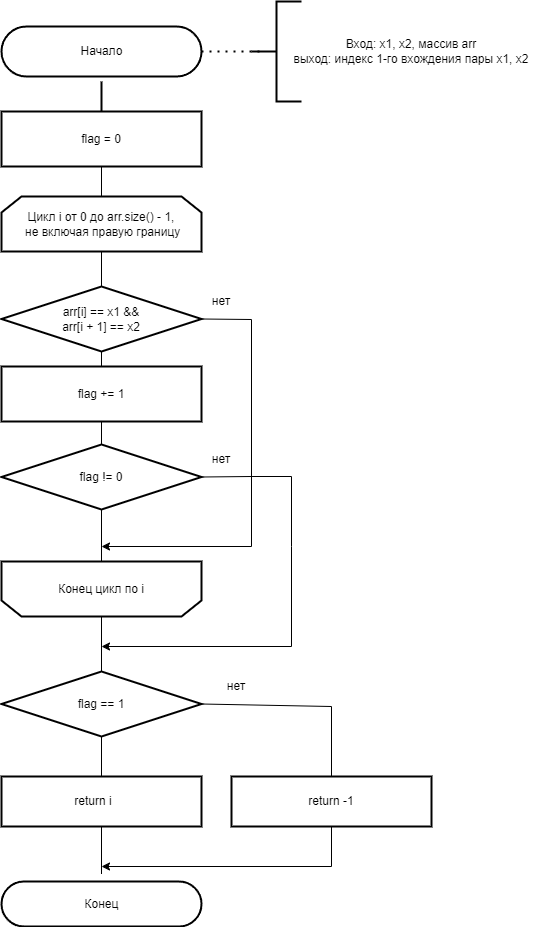
\includegraphics[scale=0.5]{img/solution.png}
	\end{center}
	\captionsetup{justification=centering}
	\caption{Aлгоритм полным перебором соседние 2 элемента}
	\label{img:solution}
\end{figure}
\clearpage
\section{Модель вычислений для оценки трудоемкости алгоритмов}

Для определения трудоемкости алгоритмов необходимо ввести модель вычислений \cite{alg1}:

\begin{enumerate}
	\item операции из списка (\ref{for:operation1}) имеют трудоемкость равную 2;
	\begin{equation}
		\label{for:operation1}
		*, /, \%, *=, /=, \%=
	\end{equation}
	\item операции из списка (\ref{for:operations2}) имеют трудоемкость равную 1;
	\begin{equation}
		\label{for:operations2}
		+, -, +=, -=, =, ==, !=, <, >, <=, >=, [], ++, {-}-
	\end{equation}
	\item трудоемкость оператора выбора \code{if условие then A else B} рассчитывается, как (\ref{for:if});
	\begin{equation}
		\label{for:if}
		f_{if} = f_{\text{условия}} +
		\begin{cases}
			f_A, & \text{если условие выполняется,}\\
			f_B, & \text{иначе.}
		\end{cases}
	\end{equation}
	\item трудоемкость цикла рассчитывается, как (\ref{for:cycle});
	\begin{equation}
		\label{for:cycle}
		f_{for} = f_{\text{инициализации}} + f_{\text{сравнения}} + N(f_{\text{тела}} + f_{\text{инкремент}} + f_{\text{сравнения}})
	\end{equation}
	\item трудоемкость вызова функции равна 0.
\end{enumerate}
\clearpage
\section{Трудоемкость алгоритмов}

Трудоемкость данного алгоритма будет складываться из следующих:

\begin{itemize}
	\item трудоемкости создания флаг, равной $1$;
	\item трудоемкости инициализации и сравнения цикла, равной $4$;
	\item трудоемкости тела, инкремента и сравнения цикла по $i$ в каждой итерации, равной $10$;
	\item трудоемкости выходного условия для функции, равной $1$;
\end{itemize}

В худшем случае --- количество итераций в цикле будет максимально, это ситуация, когда элементы исходного массива различны и не нашел результат или результат находится в конце массива. 
В этом случае трудоемкость алгоритма равна:
\begin{equation}
	\label{for:m1}
	{f^\wedge_{A}}(n) = 1 + 4 + (N - 1) \cdot 10 + 1 = 10 \cdot N - 4 = O(N)
\end{equation}

В лучшем случае --- количество итераций в цикле будет минимально, это ситуация, когда элементы исходного массива различны и результат находится в начале массива. 
В этом случае трудоемкость алгоритма равна:
\begin{equation}
	\label{for:m2}
	{f^\vee_{A}}(n) = 1 + 4 + 10 + 1 = 16 = О(1)
\end{equation}

В среднем случае. Пусть алгоритм поиска без выполнения цикла затрачивает $k_0 = 6$ операций, а при каждой итерации $k_1 = 10$ операций. алгоритм нашёл элементы на первом сравнении (лучший случай), тогда будет затрачено $k_0 + k_1$ операций, на втором --- $k_0 + 2\cdot k_1$, на последнем (худший случай) --- $k_0 + (N - 1) \cdot k_1$. Если такие элементы нет в массиве, то это, только перебрав все элементы, таким образом трудоёмкость такого случая равно трудоёмкости худшем случае.

Средняя трудоёмкость алгоритма может быть рассчитана как математическое ожидание по формуле \ref{multline} ($\Omega$ - множество всех возможных исходов).

\begin{multline}
	\label{multline}
	\sum\limits_{i \in \Omega} p_i \cdot f_i = (k_0 + k_1) \cdot \frac{1}{N + 1} + (k_0 + 2 \cdot k_1) \cdot \frac{1}{N+1} + (k_0 + 3 \cdot k_1) \cdot \frac{1}{N + 1} + \\+ (k_0 + (N - 1) \cdot k_1)\frac{1}{N + 1} + (k_0 + (N - 1) \cdot k_1) \cdot \frac{1}{N + 1} = \\= k_0\frac{N+1}{N+1}+k_1+\frac{1 + 2 + \cdots + N - 1 + N - 1}{N + 1} = k_0 + k_1 \cdot \left(\frac{N - 3}{N + 1} + \frac{N}{2}\right) =\\= k_0 + k_1 \cdot \left(1 + \frac{N}{2} - \frac{4}{N + 1}\right) = 6 + 10 \cdot \left(1 + \frac{N}{2} - \frac{4}{N + 1}\right) = O(N)
\end{multline}

\section{Требования к программному обеспечению}
К программе предъявляются следующие требования:
\begin{itemize}
	\item входные данные --- массив целых чисел, 2 разные число $x_1$ и $x_2$, $x_1$ < $x_2$;
	\item выходные данные --- индекс в массив, если найти результат, иначе -1.
\end{itemize}

\section*{Вывод}
Были представлены схемы алгоритмов поиска полным перебором ищет соседние 2 элемента и требования к программному обеспечению.
Проведённая теоретическая оценка трудоемкости алгоритмов показала, что в трудоёмкость выполнения данного алгоритма равна $O(N)$ в худшем случае, $O(1)$ в лучшем случае и $O(N)$ в среднем случае.